\chapter{A Refresher on How to Use The
Microscope}\label{a-refresher-on-how-to-use-the-microscope}

A \href{https://en.wikipedia.org/wiki/Microscope}{microscope} (from the
Ancient Greek: mikrós, ``small'' and skopeîn, ``to look'' or ``see'') is
an instrument used to see objects that are too small to be seen by the
naked eye. Microscopic means invisible to the eye unless aided by a
microscope.

There are many types of microscopes, and they may be grouped in
different ways. One way is to describe the way the instruments interact
with a sample to create images, either by sending a beam of light or
electrons to a sample in its optical path, or by scanning across, and a
short distance from, the surface of a sample using a probe. The most
common microscope (and the first to be invented) is the
\href{https://en.wikipedia.org/wiki/Optical_microscope}{optical
microscope}, which uses light to pass through a sample to produce an
image.

The objective lens of a microscope (Figure \ref{fig:objectives}) is a
cylinder containing one or more lenses that are typically made of glass.
It is essentially a high-powered magnifying glass which is brought very
close to the specimen being examined. The objective collects light from
the sample so that it comes to a focus inside the microscope tube. This
creates an enlarged image of the specimen.

\begin{figure}

{\centering 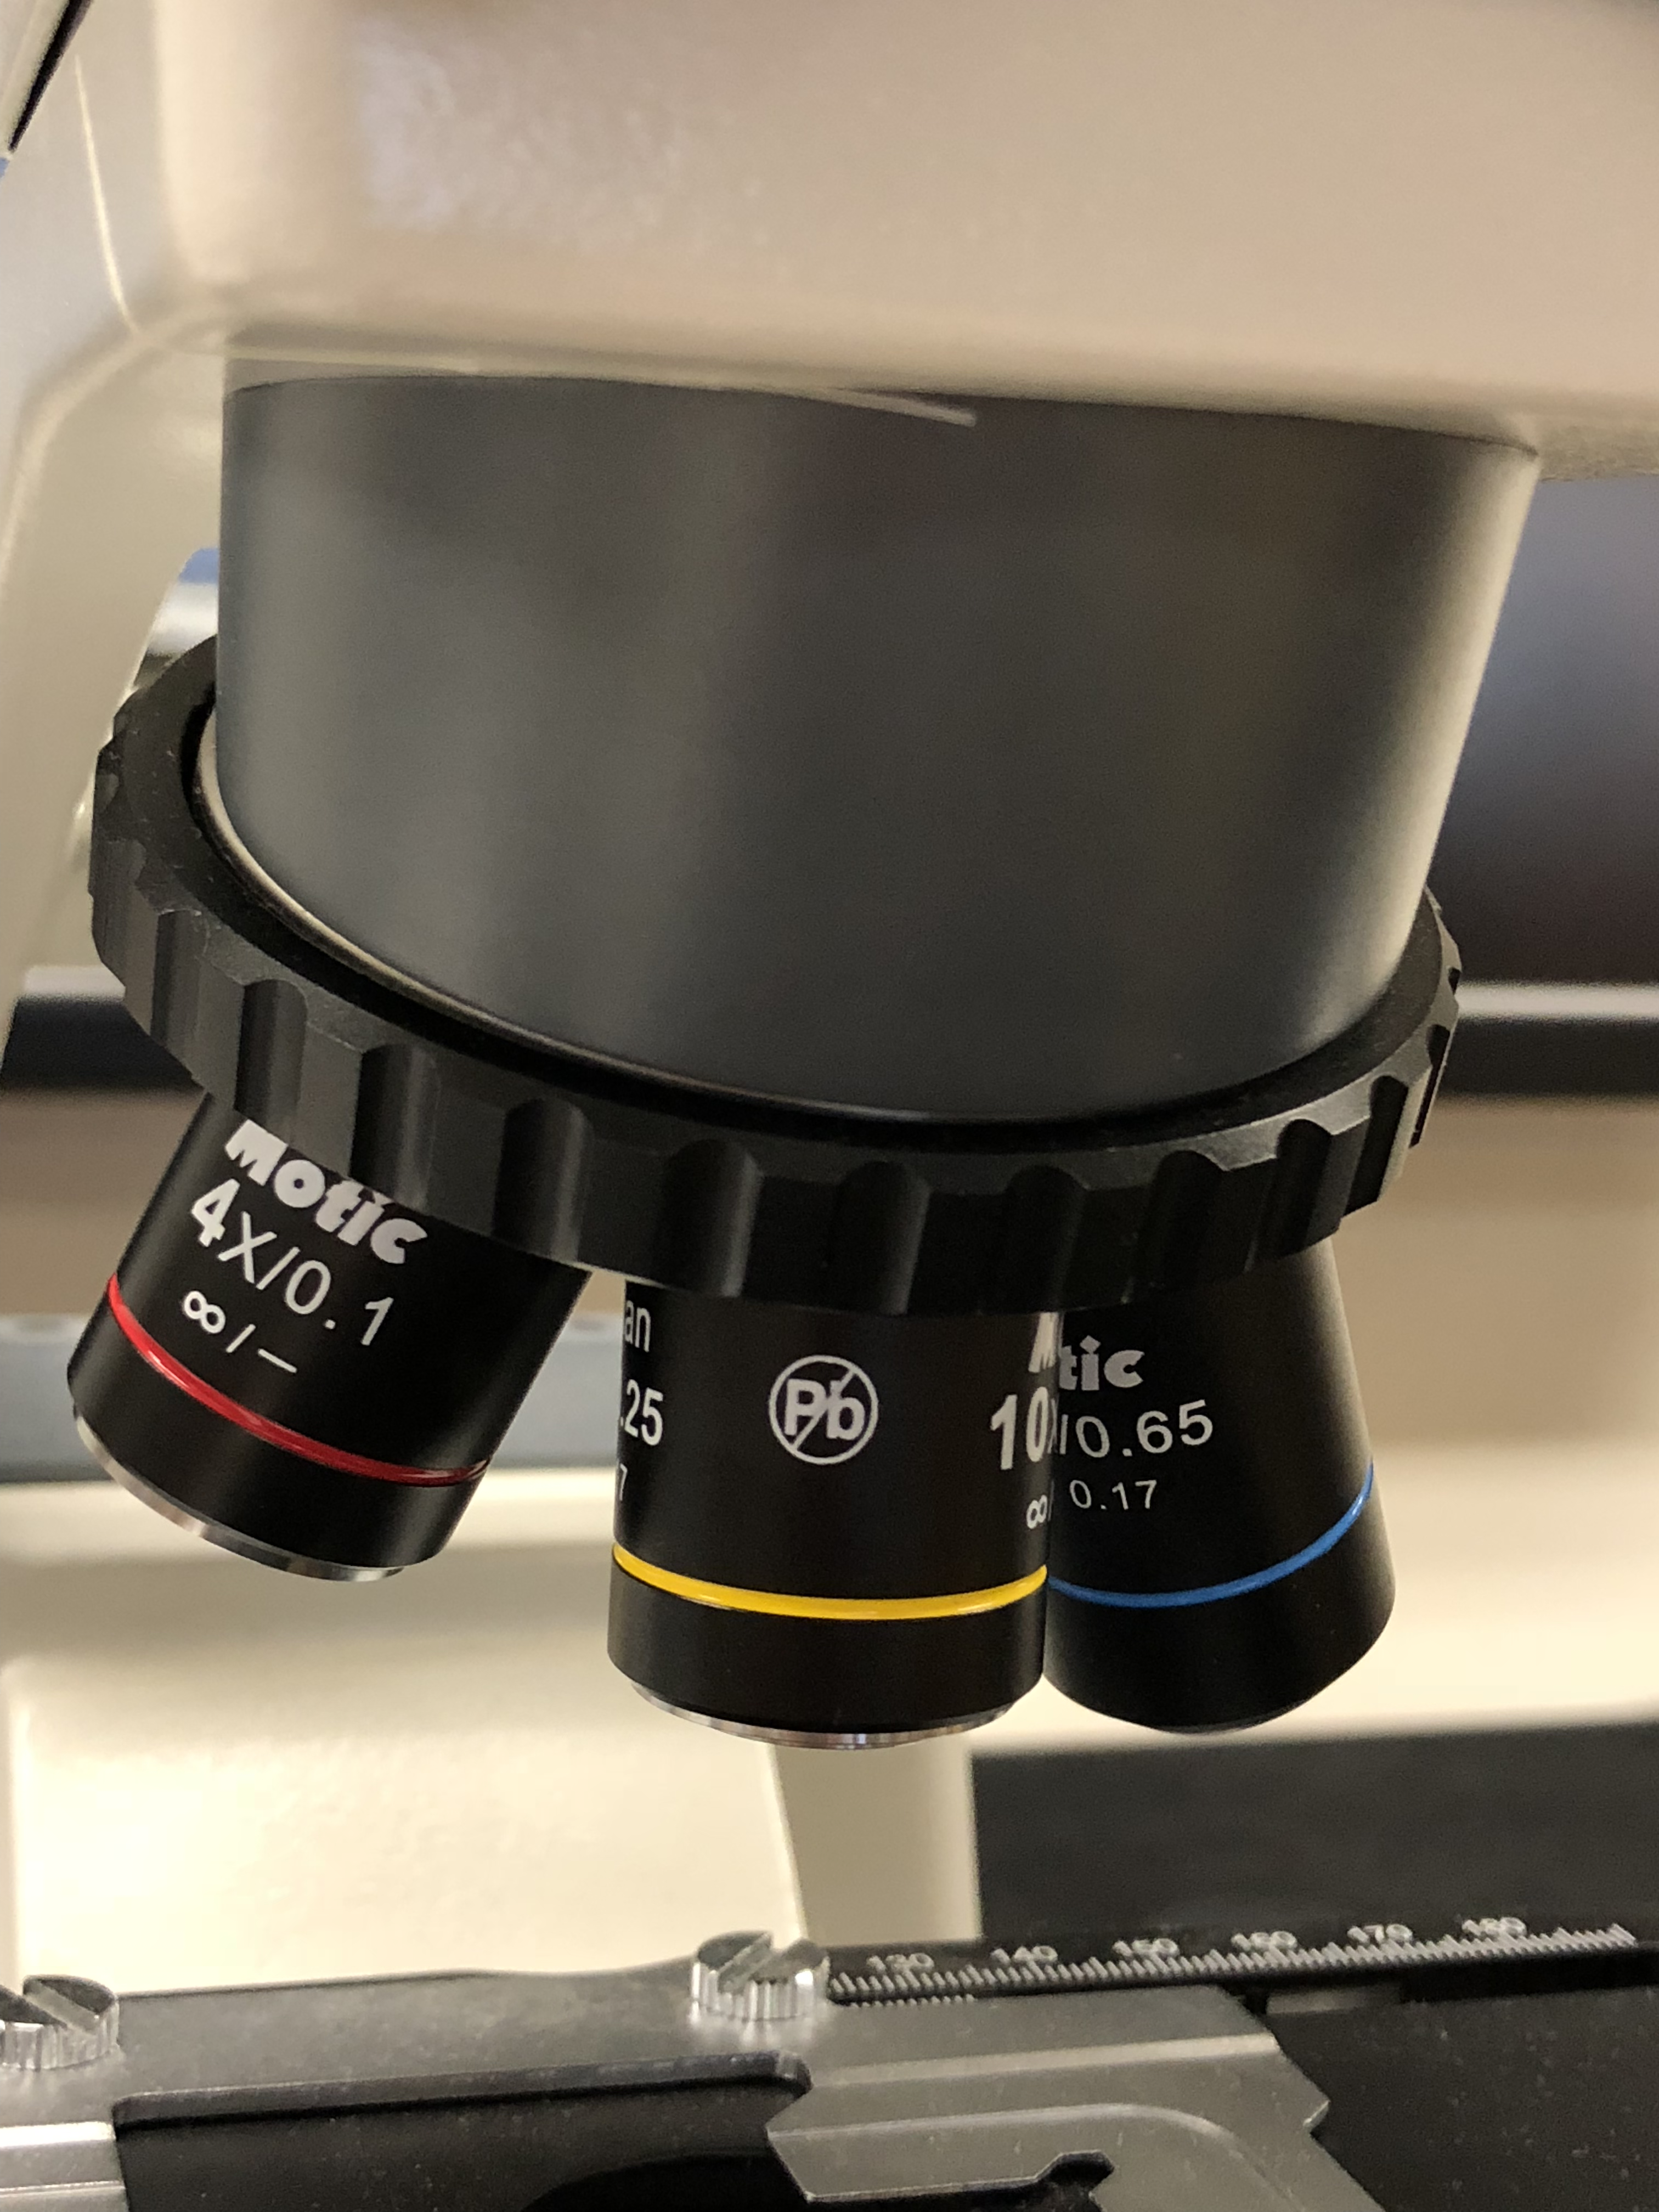
\includegraphics[width=0.7\linewidth]{./figures/microscope/Microscope_objectives}

}

\caption{The microscope objectives.}\label{fig:objectives}
\end{figure}

The eyepieces, or ocular lenses (Figure \ref{fig:oculars}), are the
lenses that are closest to your eyes when you look through the
microscope. The objective lens or mirror collects light and brings it to
focus creating an image. The eyepiece is placed near the focal point of
the objective to magnify this image. This image is inverted and can be
seen by removing the eyepiece and placing a piece of tracing paper over
the end of the tube. By carefully focusing a brightly lit specimen, a
highly enlarged image can be seen. It is this real image that is viewed
by the eyepiece lens that provides further enlargement. The amount of
magnification depends on the focal length of the eyepiece. The ocular in
our microscopes have a 10× magnification.

\begin{figure}

{\centering 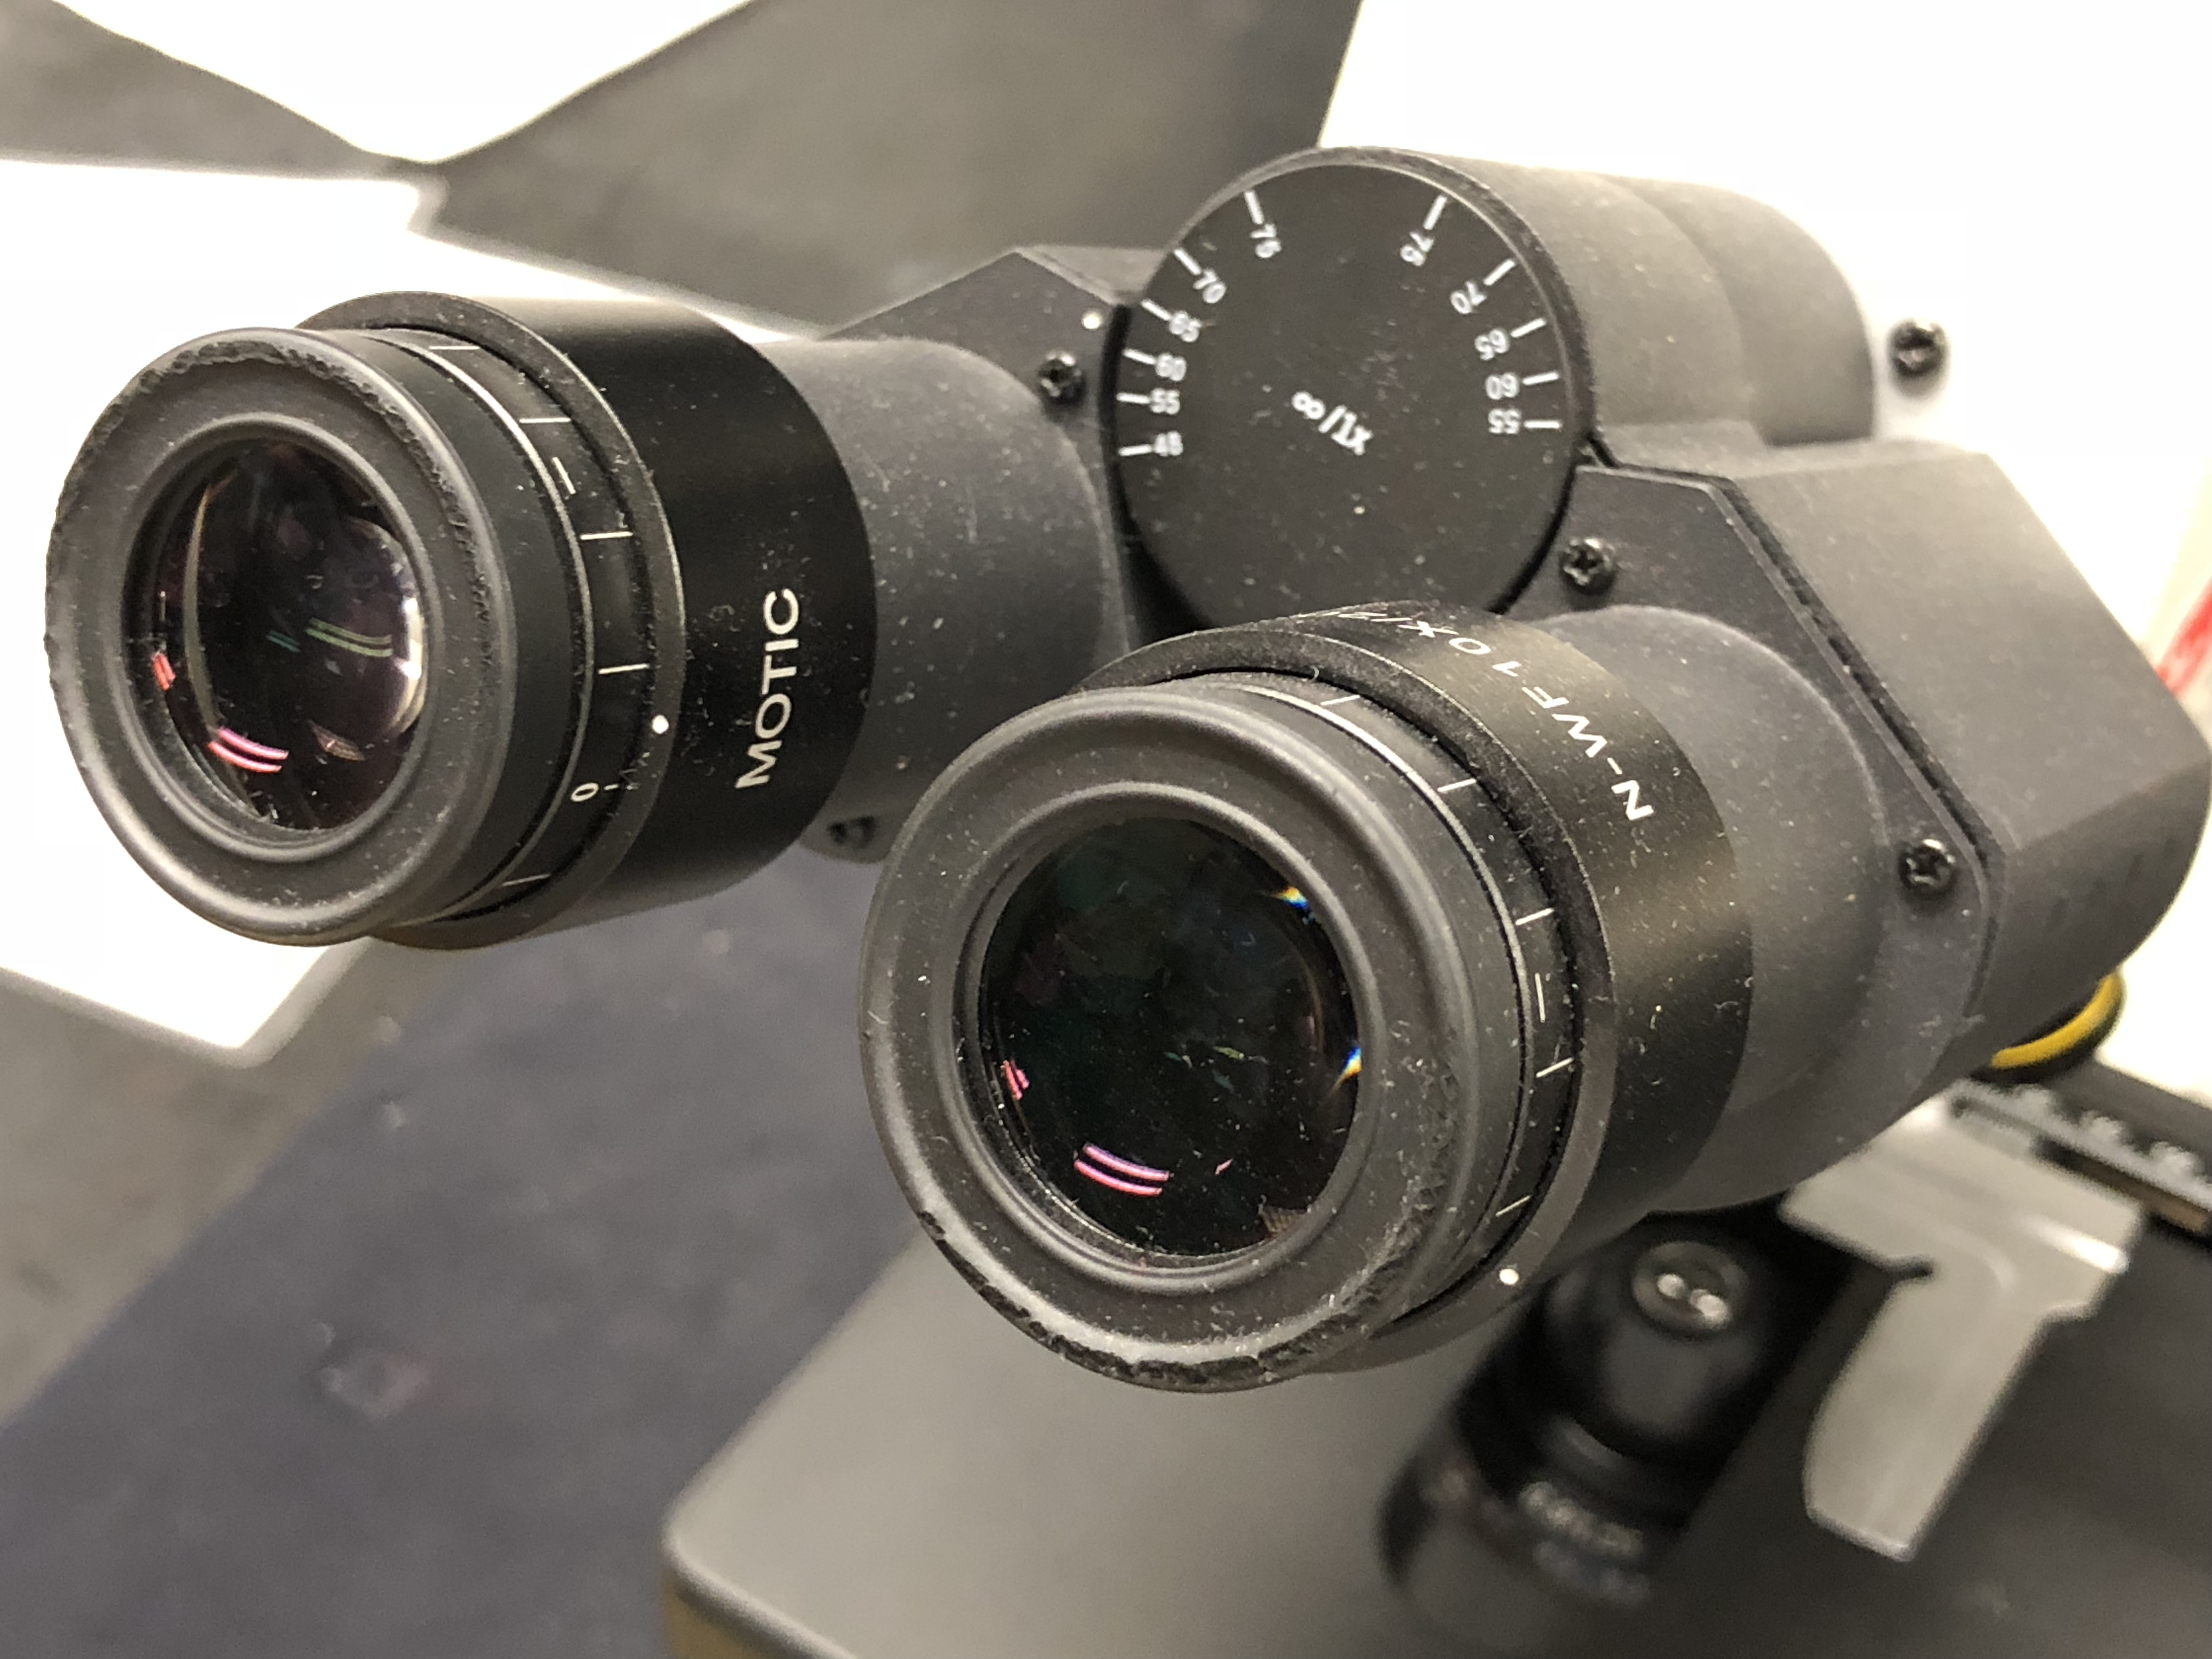
\includegraphics[width=0.7\linewidth]{./figures/microscope/Oculars}

}

\caption{The oculars (eye pieces) of the microscope.}\label{fig:oculars}
\end{figure}

Our microscopes have four objective lenses with different
magnifications, screwed into the circular ``nosepiece'' which you rotate
to select the required lens. These lenses are color coded for easier
use. The least powerful lens is called the scanning objective lens and
is a 4× objective. The second lens is referred to as the small objective
lens and is 10× lens. The most powerful lens out of the four are
referred to as the large objective lenses and are 40× and 100×. The 100×
objective is an oil-immersion lens. This objective is specially designed
for use with refractive index matching oil, which must fill the gap
between the objective lens and the specimen.

\begin{figure}

{\centering 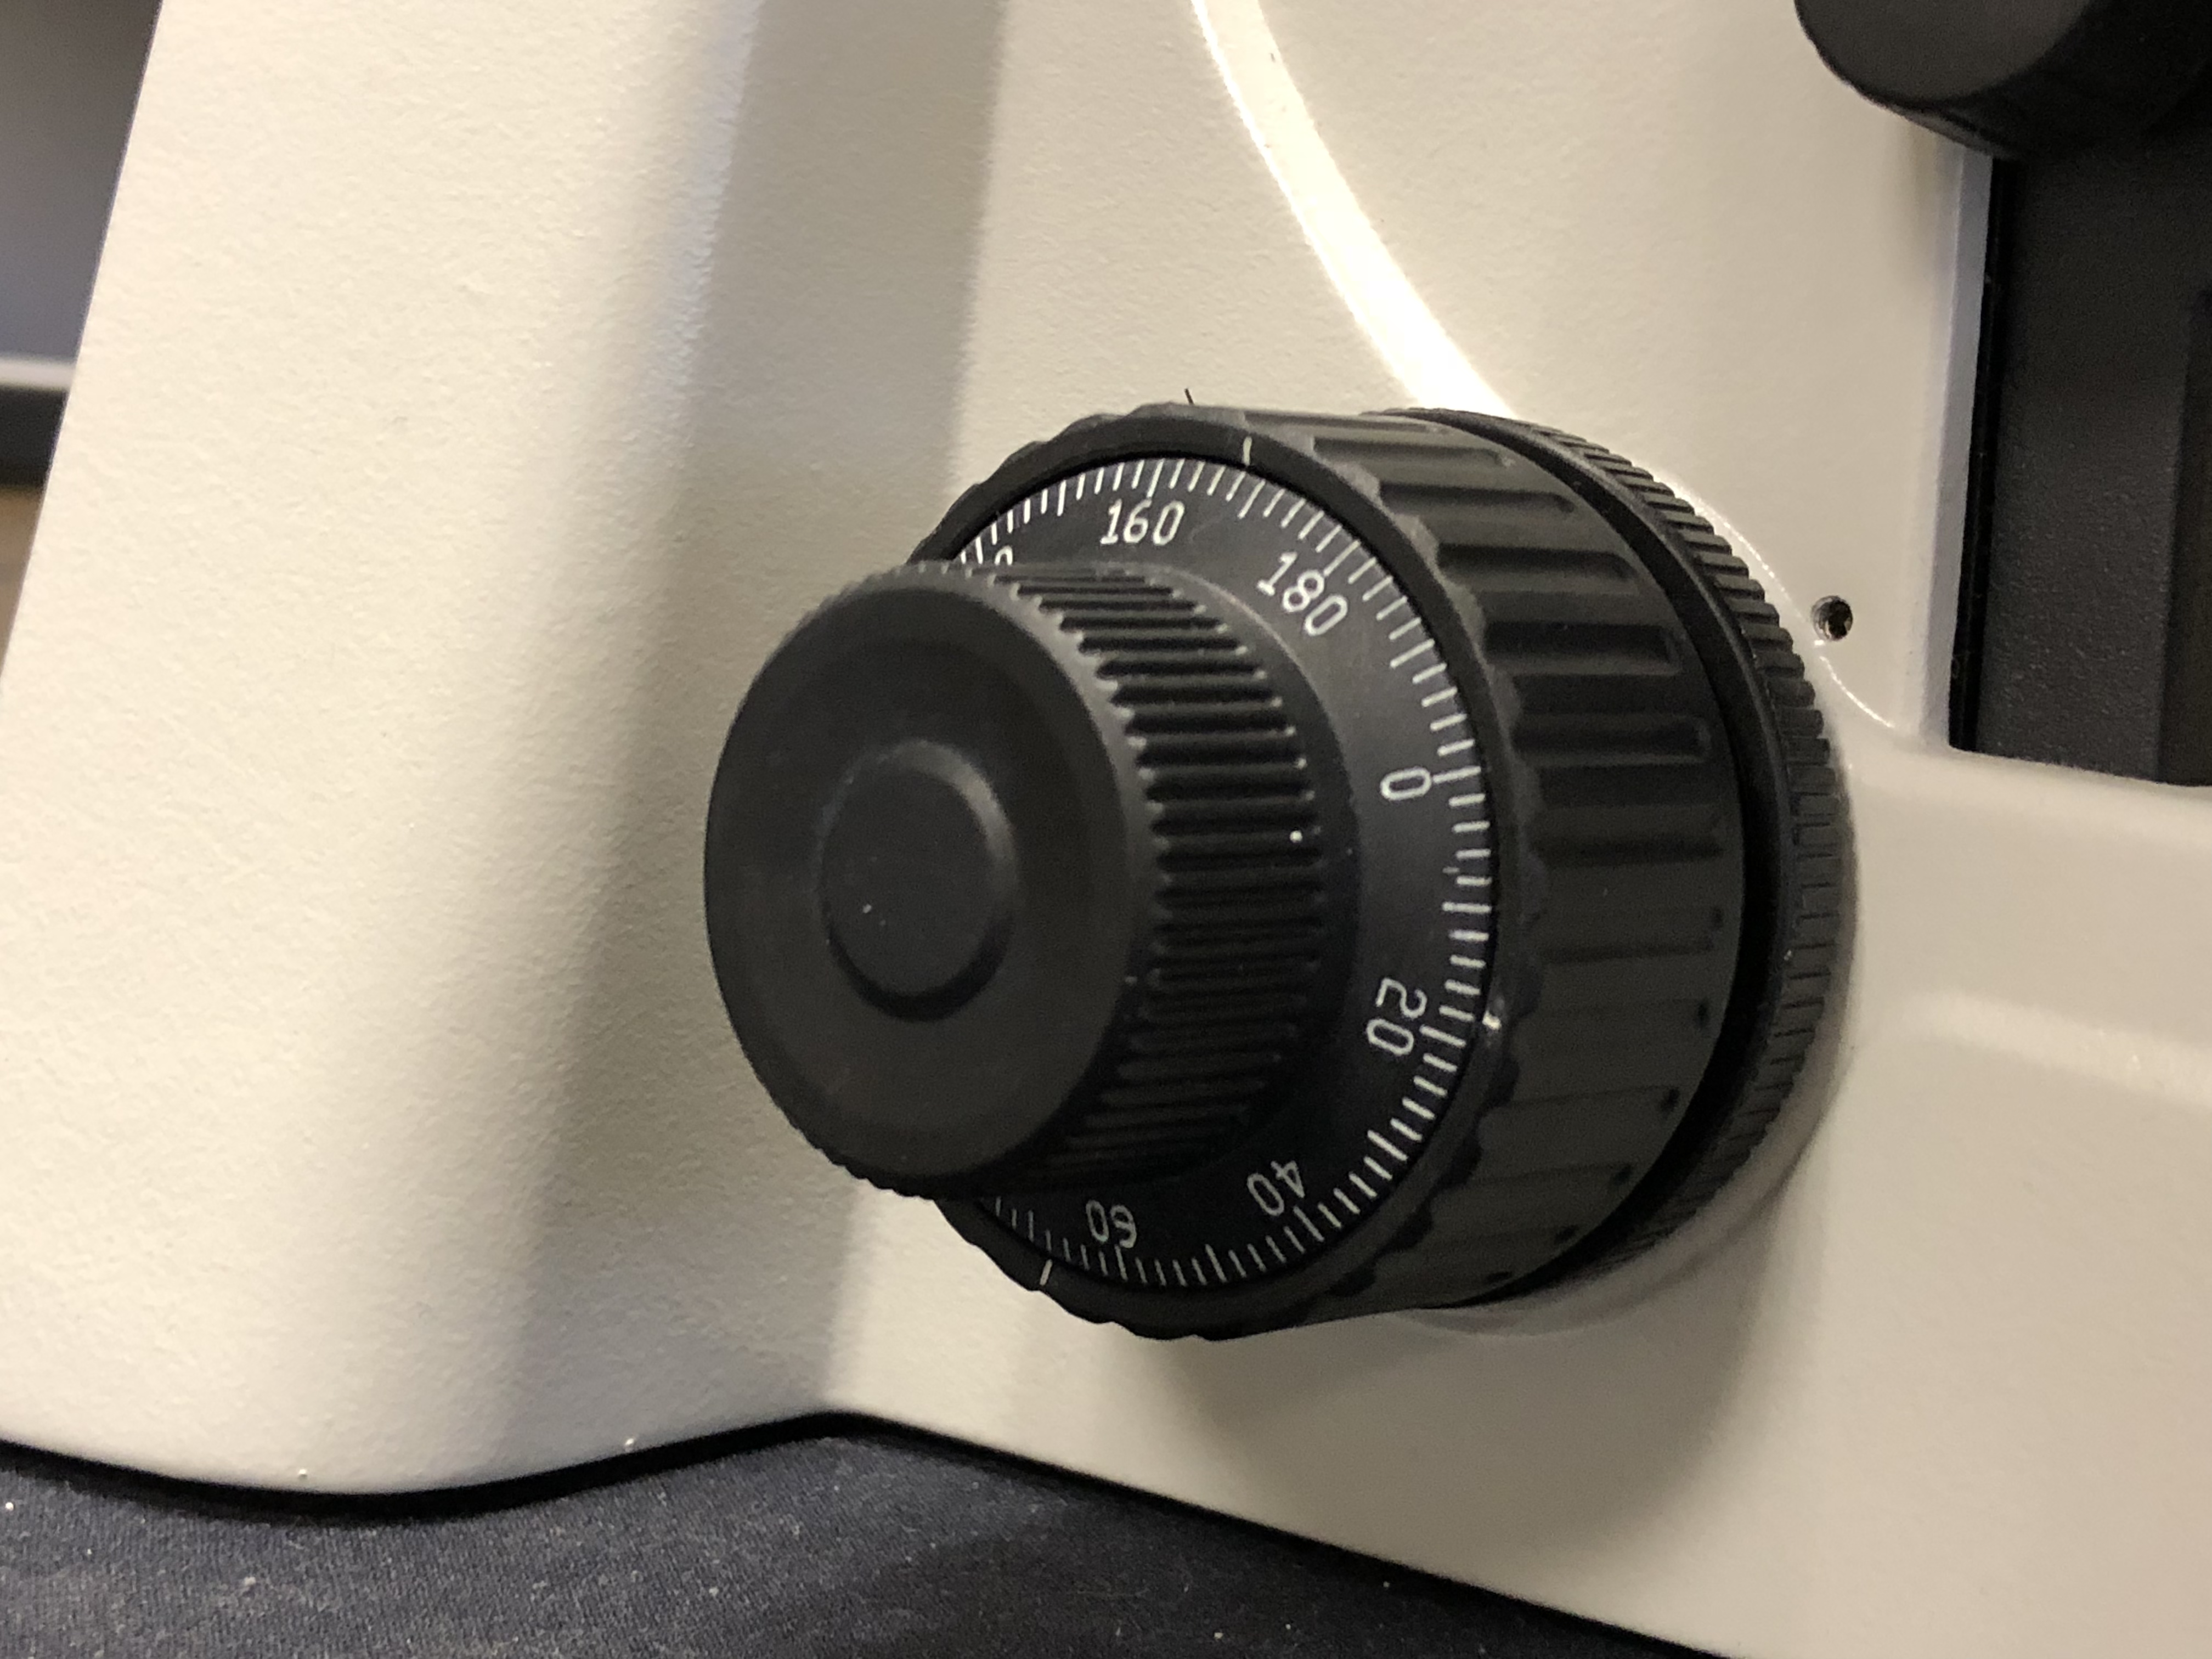
\includegraphics[width=0.7\linewidth]{./figures/microscope/focus}

}

\caption{The coarse (big wheel) and fine (small wheel) focus adjustment knobs.}\label{fig:focus}
\end{figure}

The stage is a platform below the objective which supports the specimen
being viewed. Adjustment knobs (on the left side of the microscope) move
the stage up and down with separate adjustment for coarse and fine
focusing (Figure \ref{fig:focus}). In the center of the stage is a hole
through which light passes to illuminate the specimen (Figure
\ref{fig:stage}). The stage has arms to hold slides (rectangular glass
plates on which the specimen is mounted).

\begin{figure}

{\centering 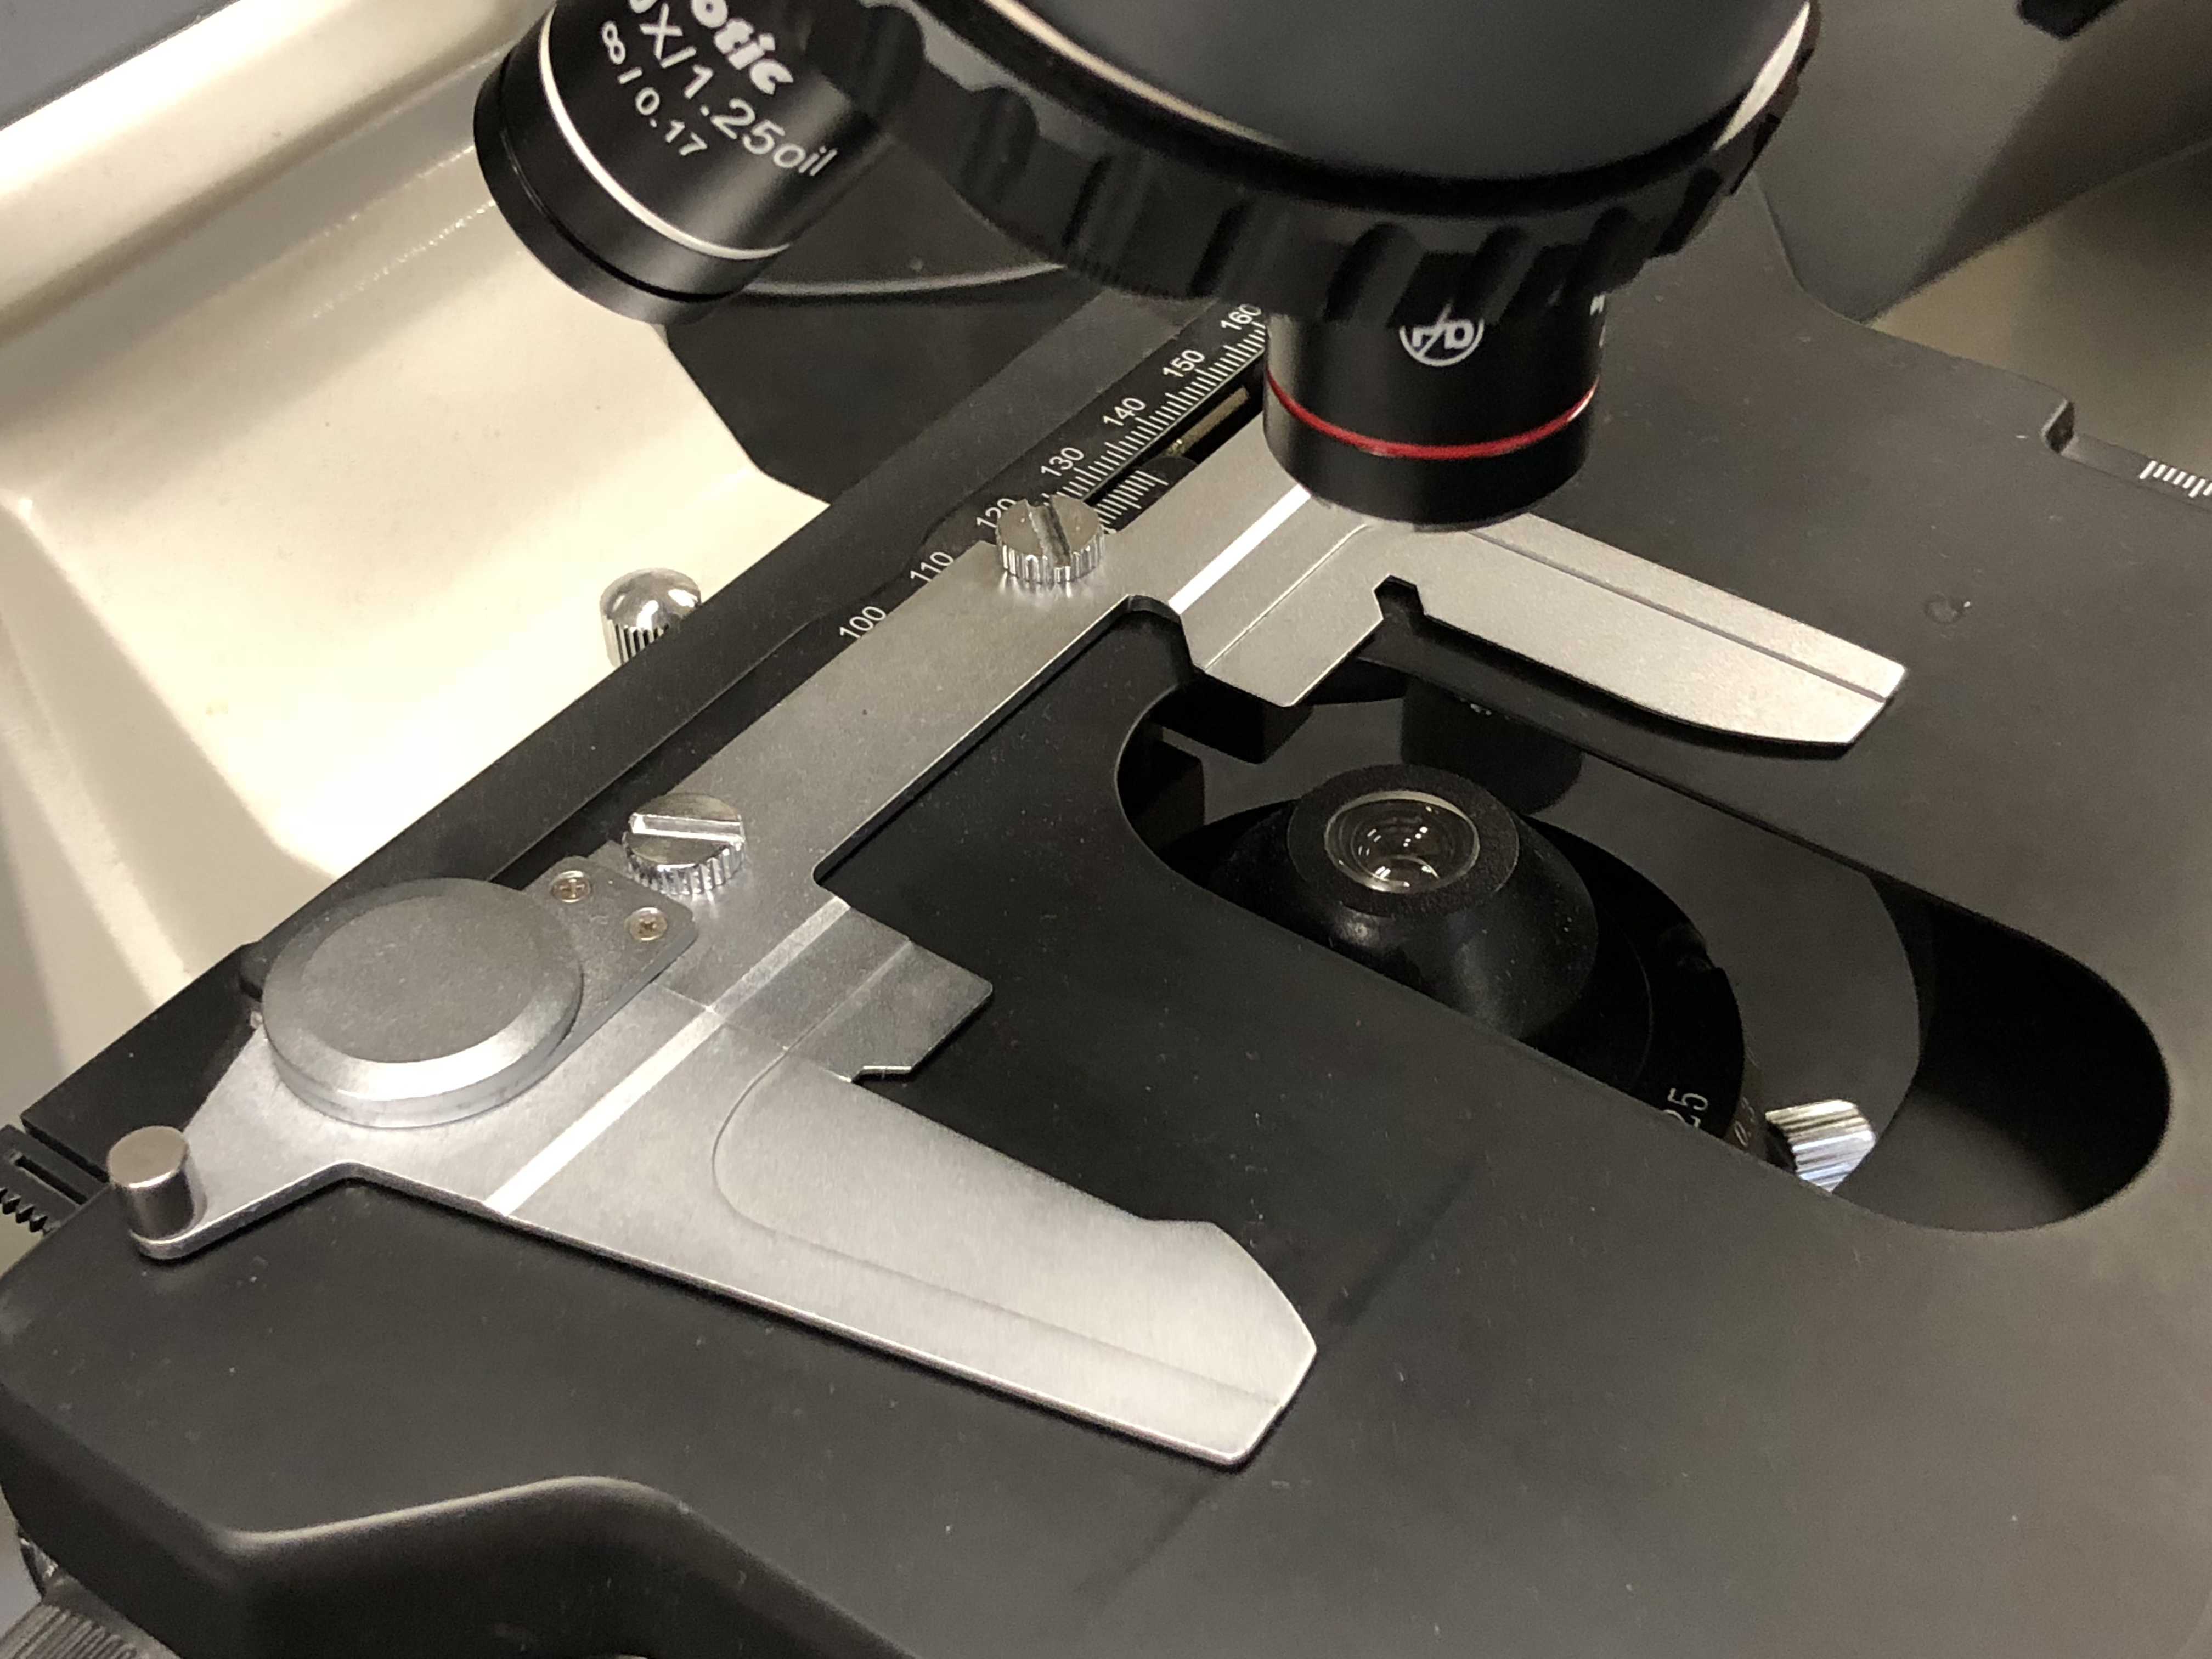
\includegraphics[width=0.7\linewidth]{./figures/microscope/stage}

}

\caption{The stage with the slide holder and central opening showing the condenser lens.}\label{fig:stage}
\end{figure}

The stage moves up and down for focus. Always start with the lowest
magnification in order to center the specimen on the stage. After moving
to a higher magnification re-focus using the fine focus knob. You may
also have to adjust the horizontal positions using the horizontal stage
and slide holder adjustment knobs hanging down on the right side of the
stage (Figure \ref{fig:condenser}). Our microscopes, an adjustable LEDs
light source (knob on the right side). The condenser is a lens designed
to focus light from the illumination source onto the sample. The light
source and condenser also each include a diaphragm to influence the
quality and intensity of the illumination. For our purposes, the
diaphragms should always be completely open. Adjust the light intensity
only using the knob on the right side of the frame of the microscope
(the black knob below the green switch in Figure \ref{fig:stage}.

\begin{figure}

{\centering 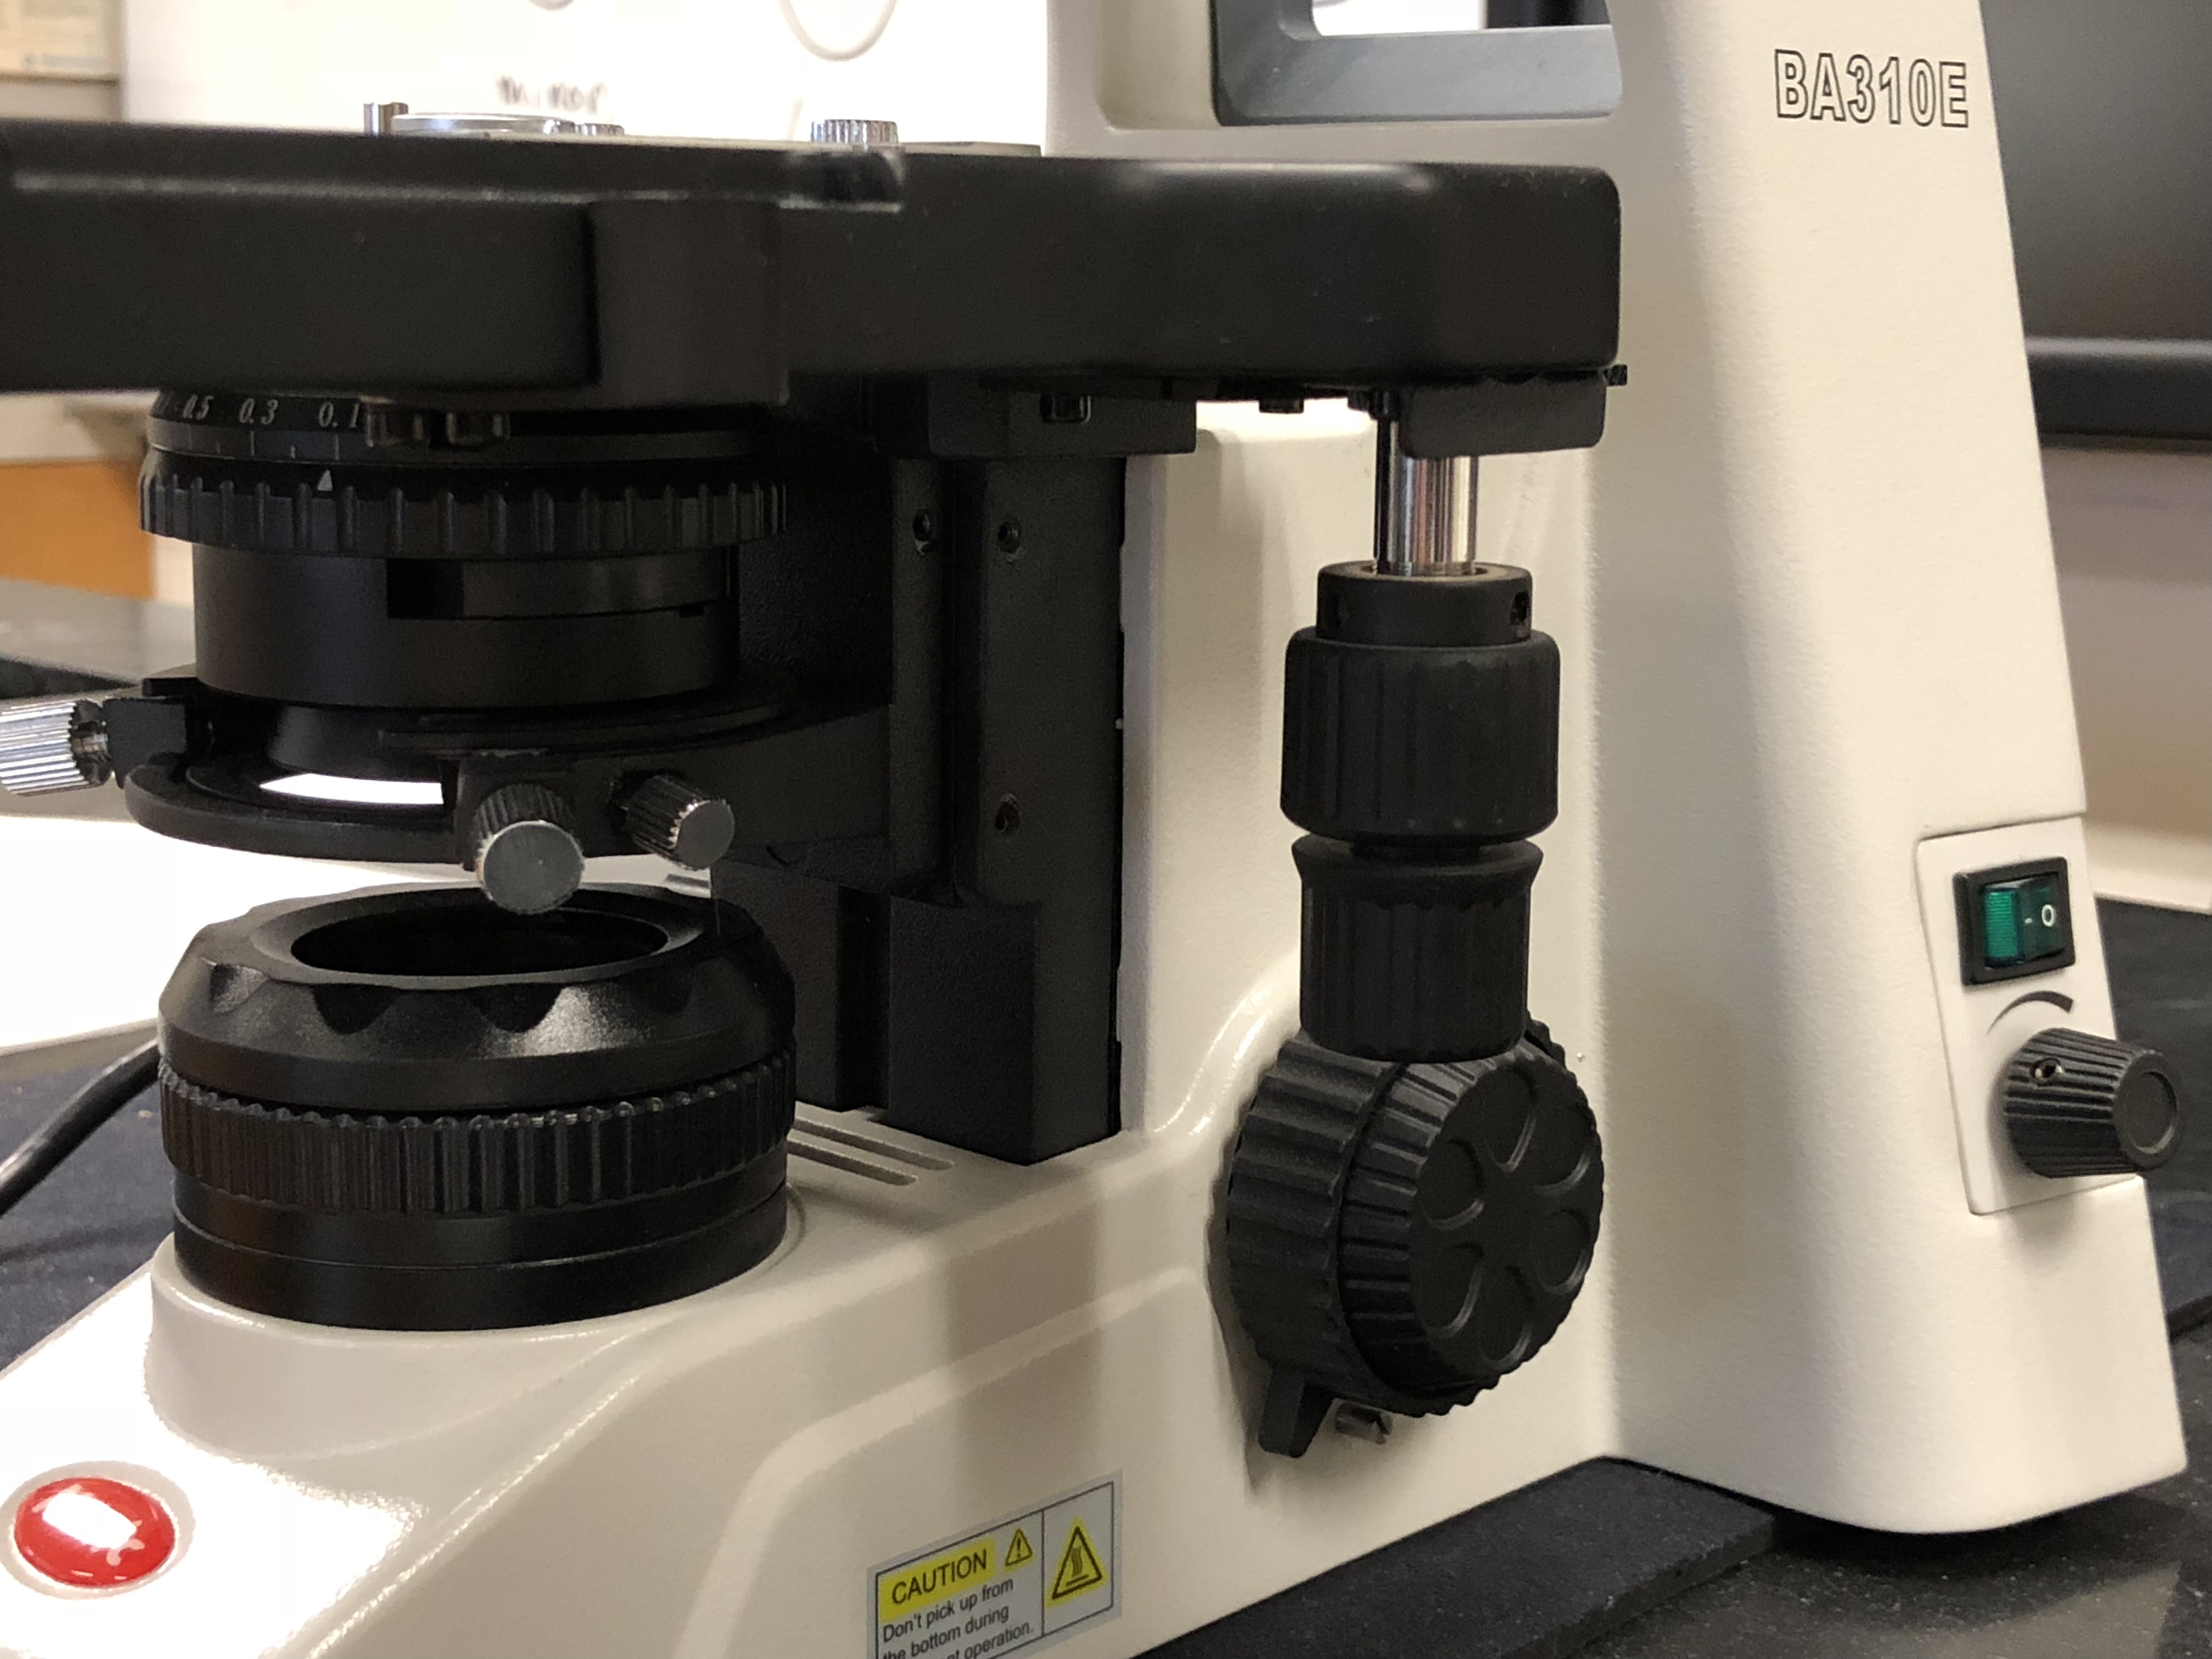
\includegraphics[width=0.7\linewidth]{./figures/microscope/condenser}

}

\caption{The condenser (below the stage), the horizontal stage and slide holder adjustment knobs (hanging down from the stage), the light on switch and light intensity adjustment knob (in the back).}\label{fig:condenser}
\end{figure}

We have prepared a number of videos that introduce our microscopes to
you and also demonstrate how you can capture images of the slides that
you are viewing and transfer them to your own equipment.

\href{https://youtu.be/2bRc3u9PMDA}{Name of Video Youtube address Introduction to microscope}


\href{https://youtu.be/qQKLu4ULRM}{Description of student and instructor microscope}


\href{https://youtu.be/wOB2BSQBZFA}{Turn on tablet and view slide}

\href{https://youtu.be/jdx1SR5dvJc}{Student image capture option 1}

\href{https://youtu.be/v5w-yuL8vg0}{Student image capture option 2}

\section{Starting up the microscope}\label{starting-up-the-microscope}

The tablets and microscopes must be turned on in a specific order:

\begin{enumerate}
\def\labelenumi{\arabic{enumi}.}
\tightlist
\item
  The microscope must be plugged in. If already plugged in, proceed to
  step 3.
\item
  The Motic logo will appear on tablet. After a few seconds, the
  charging symbol appears.
\item
  Press and hold the power button on the tablet for 6 seconds.
\item
  The Motic symbol will appear again and tablet will start up.
\item
  Turn on the microscope using the switch on the lower right side.
\end{enumerate}

\section{Turning off the microscope}\label{turning-off-the-microscope}

The tablets and microscopes must be turned off in a specific order:

\begin{enumerate}
\def\labelenumi{\arabic{enumi}.}
\tightlist
\item
  Turn off the microscope using the switch on the lower right side.
\item
  While the microscope is still plugged in, turn off the tablet by
  holding the power button down for a few seconds. Select power off.
\item
  The Motic logo will appear on tablet.
\item
  Wait until the charging symbol appears.
\item
  Leave the microscope on the student bench and plugged in after turning
  it off.
\item
  Place the cover over the microscope.
\end{enumerate}
